\begin{frame} [fragile]
	\frametitle{Experimental setup}
	\begin{columns}
  		\begin{column}{0.50\textwidth}
            \begin{itemize}
                \item The light produced in the bars is collected at each end.
                \item Each group of four SiPMs provides a single summed analogical signal.
                \item The output signal of each side of each bar was input to a waveform digitizer board, WaveDREAM, hosted in the WaveDAQ integrated trigger and data acquisition system.
            \end{itemize}
		\end{column}
    \begin{column}{0.50\textwidth}
 		\newline
			\begin{figure}
	  		    \centering
				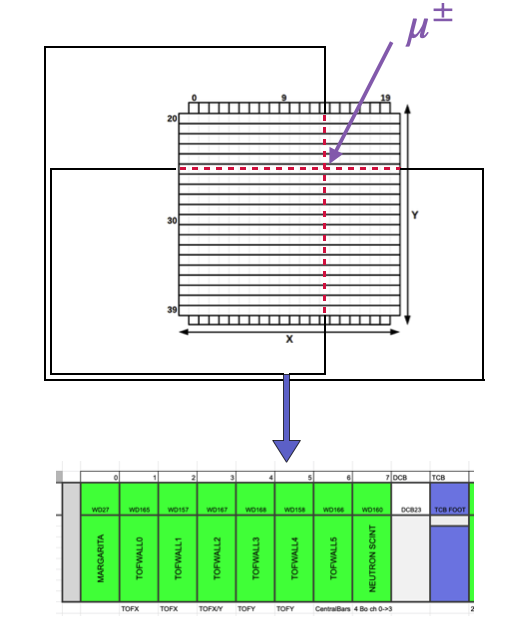
\includegraphics[scale=0.25]{figures/setup.png}
				%\caption{Spettri energetici di diversi ioni nei GCR \cite{saggiatore}}
                \caption{Thanks M. Morrocchi!}
			\end{figure}
    \end{column}
\end{columns}
\end{frame}